\documentclass[12pt,a4paper]{article}
\usepackage[utf8]{inputenc}
\usepackage[french]{babel}
\usepackage[T1]{fontenc}
\usepackage{amsmath}
\usepackage{amsfonts}
\usepackage{amssymb}
\usepackage{graphicx}
\usepackage{geometry}
\usepackage{hyperref}
\usepackage{titlesec}
\usepackage{booktabs}
\usepackage{xcolor}
\usepackage{listings}
\usepackage{caption}
\usepackage{float}

\geometry{margin=2.5cm}

% --- Custom Colors ---
\definecolor{primary}{RGB}{31, 111, 235}
\definecolor{secondary}{RGB}{13, 17, 23}

\hypersetup{
    colorlinks=true,
    linkcolor=black,
    filecolor=magenta,      
    urlcolor=primary,
    pdftitle={Rapport Mini-Projet - Détection URL},
}

% --- Title Page ---
\begin{document}

\begin{titlepage}
    \centering
    \vspace*{1cm}
    {\Huge \textbf{Mini-Projet}} \\
    \vspace{0.5cm}
    {\LARGE \textbf{Détection d’URL Malveillantes par IA}} \\
    \vspace{1.5cm}
    \includegraphics[width=0.4\textwidth]{esi_logo.png} \\ % Assuming you have the logo
    \vspace{1.5cm}
    {\large \textbf{Module : Sécurité des Données 2SC IASD}} \\
    \vspace{2cm}
    \textbf{Groupe :} \\
    \begin{tabular}{ll}
        \textbf{Nom} & \textbf{Prénom} \\
        MIHI & Badis Mohammed Ali \\
        KAID & Akram \\
        SENNOUCI & Abdeldjalil Kouider \\
        MAZARI & Amine Abdessamed \\
    \end{tabular} \\
    \vspace{2cm}
    \textbf{Lien Dashboard :} \\
    \href{https://minip-sec-detection-cterzjd4qymadkqxbyqytx.streamlit.app}{Accéder à l'application en direct} \\
    \vfill
    \textbf{Date de remise :} \today
\end{titlepage}

\newpage
\tableofcontents
\newpage

\section{Introduction}
\subsection{Contexte du projet}
La détection d'URL malveillantes est un pilier fondamental de la cybersécurité moderne. Avec l'augmentation exponentielle des cyberattaques, les méthodes traditionnelles basées sur les listes noires ne suffisent plus. Ce projet propose une approche basée sur l'apprentissage automatique (Machine Learning) pour classifier en temps réel les menaces web.

\subsection{Problématique}
Comment identifier avec précision et rapidité une URL malveillante (Phishing, Malware, Defacement) parmi des millions de requêtes, tout en minimisant les faux positifs qui bloqueraient des sites légitimes ?

\subsection{Objectifs du projet}
\begin{itemize}
    \item Développer un pipeline complet de traitement de données (cleaning, extraction).
    \item Implémenter et comparer des modèles ML (Random Forest, XGBoost) et DL (LSTM).
    \item Déployer une solution interactive via Streamlit pour une démonstration pratique.
\end{itemize}

\section{Jeu de Données et Analyse Exploratoire}
\subsection{Présentation du dataset ISCX-URL2016}
Nous utilisons le dataset ISCX-URL2016, une référence académique contenant plus de 650,000 URL étiquetées.
\begin{table}[H]
\centering
\caption{Distribution des classes dans le projet}
\begin{tabular}{@{}ll@{}}
\toprule
\textbf{Classe} & \textbf{Description} \\ \midrule
Benign & URL saine et sûre. \\
Phishing & Tentative d'usurpation d'identité. \\
Malware & Site hébergeant des logiciels malveillants. \\
Defacement & Site défiguré par un pirate. \\ \bottomrule
\end{tabular}
\end{table}

\section{Méthodologie}
\subsection{Aperçu général du pipeline}
Le système suit un flux rigoureux : Chargement $\rightarrow$ Nettoyage $\rightarrow$ Extraction Hybride $\rightarrow$ Entraînement $\rightarrow$ Évaluation.

\subsection{Prétraitement des données}
\begin{itemize}
    \item \textbf{Nettoyage} : Suppression des protocoles redondants et conversion en minuscules.
    \item \textbf{Normalisation} : Standardisation des caractéristiques numériques.
\end{itemize}

\section{Ingénierie des Caractéristiques}
\subsection{Extraction Hybride}
Nous avons opté pour une approche combinée :
\begin{enumerate}
    \item \textbf{TF-IDF} : Analyse fréquentielle des caractères pour capturer les motifs textuels.
    \item \textbf{Handcrafted Features} : 11 caractéristiques structurelles (Longueur, présence de caractères spéciaux, HTTPS, etc.).
\end{enumerate}

\subsection{Importance des caractéristiques}
\begin{figure}[H]
    \centering
    %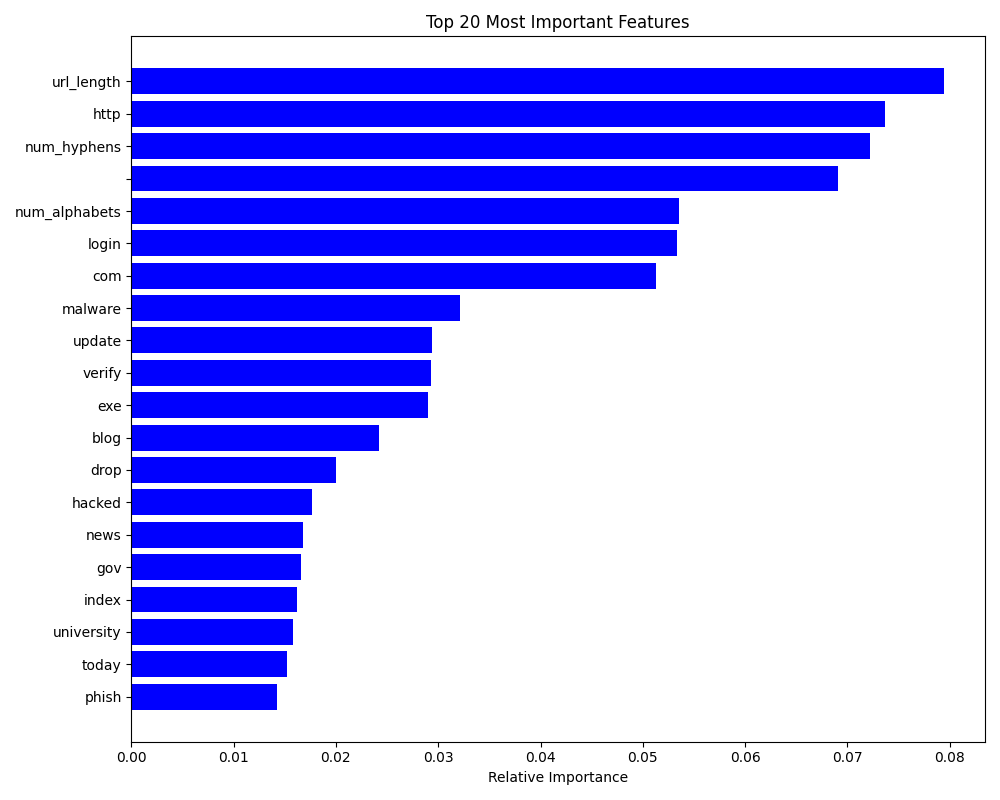
\includegraphics[width=0.8\textwidth]{plots/feature_importance.png}
    \caption{Top 20 des caractéristiques les plus discriminantes (Modèle Random Forest)}
\end{figure}

\section{Modèles d’Apprentissage}
\subsection{Algorithmes de Machine Learning}
\begin{itemize}
    \item \textbf{Random Forest (RF)} : Notre modèle principal, offrant le meilleur compromis précision/rapidité.
    \item \textbf{XGBoost} : Utilisé pour sa robustesse face aux données déséquilibrées.
\end{itemize}

\subsection{Modèles de Deep Learning}
\begin{itemize}
    \item \textbf{LSTM} : Pour l'analyse séquentielle des URL caractère par caractère.
\end{itemize}

\section{Résultats Expérimentaux}
\subsection{Comparaison des modèles}
Les performances ont été évaluées sur un ensemble de test (split 20\%).

\begin{table}[H]
\centering
\caption{Comparaison des performances des modèles}
\begin{tabular}{@{}lcccc@{}}
\toprule
\textbf{Modèle} & \textbf{Accuracy} & \textbf{Precision} & \textbf{Recall} & \textbf{F1-Score} \\ \midrule
\textbf{Random Forest} & \textbf{98.09\%} & \textbf{97.5\%} & \textbf{98.1\%} & \textbf{97.8\%} \\
XGBoost & 97.4\% & 96.8\% & 97.4\% & 97.1\% \\
LSTM & 96.3\% & 95.5\% & 96.3\% & 95.9\% \\
Logistic Regression & 91.7\% & 90.2\% & 91.7\% & 90.9\% \\ \bottomrule
\end{tabular}
\end{table}

\section{Aspects de Sécurité}
Le modèle permet d'identifier des attaques critiques :
\begin{itemize}
    \item \textbf{Phishing} : Détecté par l'analyse des mots-clés (login, secure) et des anomalies de domaine.
    \item \textbf{Defacement} : Identifié par des structures d'URL inhabituelles.
\end{itemize}

\section{Conclusion}
Le projet démontre qu'une approche hybride (Lexicale + Structurelle) permet d'atteindre une précision de plus de 98\%. L'intégration d'un dashboard Streamlit permet une exploitation immédiate du modèle pour la protection des utilisateurs.

\vspace{1cm}
\textbf{Lien de démonstration :} \\
\url{https://minip-sec-detection-cterzjd4qymadkqxbyqytx.streamlit.app}

\end{document}
